% ---------------------------------------------------------------
% Preamble
% ---------------------------------------------------------------
\documentclass[a4paper,11pt]{article}

\usepackage[utf8]{inputenc}
\usepackage[english]{babel}
\usepackage[margin=1in,a4paper,pdftex]{geometry}
\usepackage[protrusion=true,expansion=true]{microtype} 
\usepackage{amsmath,amsfonts,amsthm,amssymb,bm,mathdots,mathtools,bigints}
\usepackage{rotating}
\usepackage[colorlinks=true, linkcolor=blue, urlcolor=blue, anchorcolor=blue, citecolor=red]{hyperref}
\usepackage[all]{hypcap}
\usepackage{color, xcolor}
\usepackage{listings, newtxtt}
\usepackage[ruled,linesnumbered]{algorithm2e}
\usepackage{cite}
\usepackage{makecell}
\usepackage[printwatermark]{xwatermark}
\usepackage{subcaption}
\usepackage{siunitx}
\usepackage{tikz, pgfplots}

\usepackage{framed}
\definecolor{myYellow}{rgb}{1,0.65,0}
\definecolor{myRed}{rgb}{0.84, 0.18, 0.13}
\definecolor{myGreen}{rgb}{0, 0.53, 0.27}
\definecolor{myBlue}{rgb}{0, 0.34, 0.91}
\colorlet{shadecolor}{myBlue!7}

\numberwithin{figure}{section}
\numberwithin{equation}{section}
\numberwithin{table}{section}

\newtheorem{theorem}{Theorem}[section]
\newtheorem{corollary}{Corollary}[theorem]
\newtheorem{lemma}[theorem]{Lemma}

\theoremstyle{definition}
\newtheorem{definition}{Definition}[section]

%\newwatermark[allpages,color=red!15,angle=45,scale=5,xpos=-1cm,ypos=2cm]{DRAFT}

\makeatletter
\setlength{\@fptop}{0pt}
\makeatother

\usepackage{graphicx}
\graphicspath{ {figs/} }

\newbox{\bigpicturebox}

\lstset{
    backgroundcolor=\color{myBlue!7},
    language=Python, keywordstyle=\color[rgb]{0,0,1},
    basicstyle=\ttfamily, keywordstyle=\bfseries,
    escapeinside={\%*}{*)}
}

% --------------------------------------------------------------------
% Tikz Macros
% --------------------------------------------------------------------
\usetikzlibrary{shapes,arrows, backgrounds, positioning, fit, decorations.pathmorphing}

\tikzstyle{sectionBlock} = [draw, fill=blue!20, rectangle, minimum height=3em, minimum width=3em]
\tikzstyle{block} = [draw, fill=white, rectangle, minimum height=3em, minimum width=3em]
\tikzstyle{sum} = [draw, fill=white, circle, node distance=1cm]
\tikzstyle{input} = [coordinate]
\tikzstyle{output} = [coordinate]
\tikzstyle{pinstyle} = [pin edge={to-,thin,black}]
\tikzstyle{mcInput} = [draw, rectangle, line width=0.5mm, minimum width=2em, minimum height=2em, fill=black!10]
\tikzstyle{mcCircle} = [draw, circle, line width=0.5mm, minimum width=2em, minimum height=2em, fill=white]

% --------------------------------------------------------------------
% Definitions
% --------------------------------------------------------------------
\newcommand{\HRule}[1]{\rule{\linewidth}{#1}} 

\makeatletter                       
\def\printtitle{
    {\centering \@title\par}}
\makeatother                                    

\makeatletter 
\def\printauthor{
    {\centering \large \@author}}               
\makeatother                            

\newcounter{boxed-theorem}
\makeatletter
\newenvironment{boxed-theorem}[1]
{\begin{shaded} \begin{theorem}{#1}}
{\end{theorem} \end{shaded}}

\newcounter{boxed-definition}
\makeatletter
\newenvironment{boxed-definition}[1]
{\begin{shaded} \begin{definition}{#1}}
{\end{definition} \end{shaded}}

% ---------------------------------------------------------------
% Metadata 
% ---------------------------------------------------------------
\title{ \normalsize \textsc{TI0119 - PROCESSAMENTO DIGITAL DE SINAIS} 
        \\[2.0cm]             
        \HRule{0.5pt} \\              
        \LARGE \textbf{\uppercase{Transformada Rápida de Fourier}\\2º Avaliação Parcial}
        \HRule{2pt} \\[0.5cm]  
}

\author{
        Otacílio Bezerra Leite Neto\\   
        Universidade Federal do Ceará\\  
        Departamento de Engenharia de Teleinform\'atica\\
        \texttt{minhotmog@gmail.com} \\
}

\begin{document}
% ---------------------------------------------------------------
% Maketitle
% ---------------------------------------------------------------
\thispagestyle{empty}       % Remove page numbering on this page

\printtitle                 % Print the title data as defined above
    \vfill
\printauthor                % Print the author data as defined above
\newpage

% ---------------------------------------------------------------
% Begin document
% ---------------------------------------------------------------
\setcounter{secnumdepth}{1}
\setcounter{tocdepth}{1}

% 1 - Introduction
% ---------------------------------------------------------------
\clearpage
\setcounter{page}{1}
\section{Exercícios - Página 13}

\begin{shaded}
	\noindent Faça a convulação entre duas janelas de largura diferente, com valores não-nulos unitários. Uso algoritmos rápidos e o cálculo de convolução discreta para comparação.
\end{shaded}

\noindent \textbf{Resposta:}

Demonstra-se abaixo os resultados obtidos para e exercício proposto. A explicação matemática e sobrea a implementação dos algoritmos está detalhada no final deste documento. Para efeitos práticos, consideramos as duas janelas de largura diferente através das seguências $x_1[n]$ e $x_2[n]$ definidas como
\begin{equation}
	\begin{matrix}
		x_1[n] = \begin{cases} 1 & \text{se } 0 \leq n < 6 \\ 0 & \text{caso contrário}\end{cases}; &  &
		x_2[n] = \begin{cases} 1 & \text{se } 0 \leq n < 12 \\ 0 & \text{caso contrário}\end{cases}.
	\end{matrix}
\end{equation}

\noindent A segunda janela é definida como tendo o dobro de largura da primeira. Para realização dos experimentos, considerou-se um número total de $N = 2^5 = 32$ amostras discretas consecutivas dessa sequência. Uma visualização das duas sequências, no domínio do tempo discreto, é exibida na Figura \ref{fig:windows} abaixo.

\begin{figure}[ht] \centering
	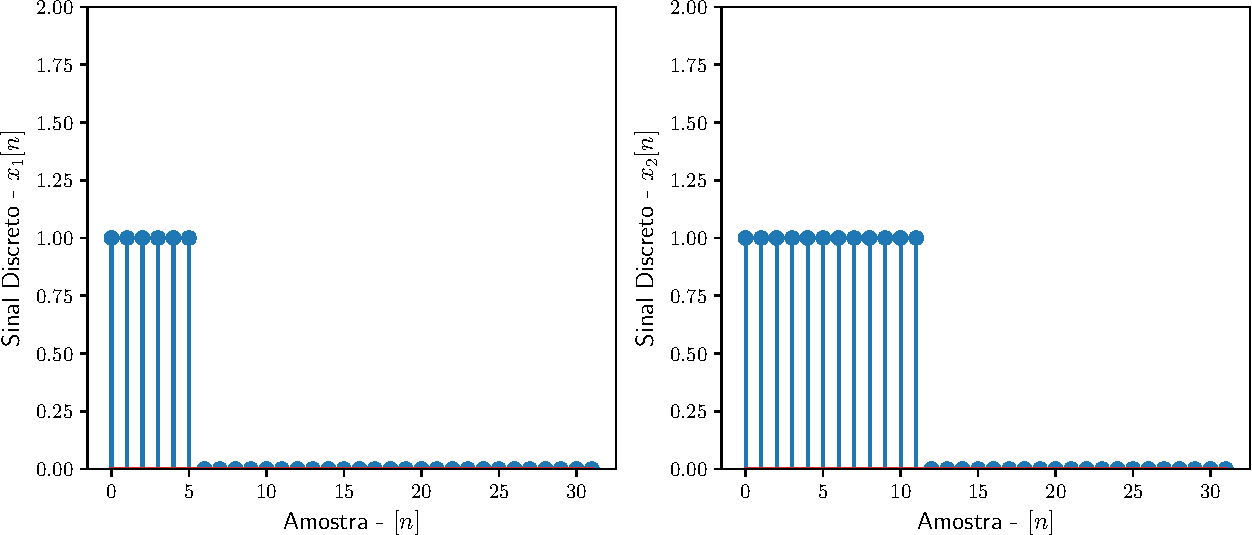
\includegraphics[width=\textwidth]{windows}
	\caption{Visualização das sequências $x_1[n]$ e $x_2[n]$.}
	\label{fig:windows}
\end{figure}

O objetivo do exercício consiste em realizar uma convolução no tempo entre esses dois sinais, ou seja, calcular $x[n] = x_1[n]*x_2[n]$. Uma famosa propriedade da Transformada de Fourier (que também é válida para transformadas discretas) estabelece que a operação de convolução, no domínio do tempo, entre dois sinais é equivalente a realizar à operação de multiplicação entre suas respectivas transformadas, no domínio da frequência. Essa propriedade pode ser denotada matematicamente:
\begin{equation}
\begin{matrix}
	x[n] = \displaystyle\sum_{m=0}^{N-1} x_1[n] x_2[n-m] \overset{\mathcal{FD}}{\rightleftharpoons} X_1[k] X_2[k] = X[k]
\end{matrix}.
\end{equation}

Portanto, é possível realizar o seguinte procedimento a fim de obter o resultado da convolução:

\begin{enumerate}
	\item Calcular as Transformadas de Fourier Discretas (DFT) para as duas sequências em questão. Denota-se às sequências no domínio da frequência, $X_1[k]$ e $X_2[k]$, a definição da transformada direta:
	\begin{equation}
	\begin{matrix}
		X_1[k] = \displaystyle\sum_{n = 0}^{N-1} x_1[n] e^{-j\frac{2\pi k}{N}n}, &
		X_2[k] = \displaystyle\sum_{n = 0}^{N-1} x_2[n] e^{-j\frac{2\pi k}{N}n}, & (k = 0,1,\cdots,N-1).
	\end{matrix}
	\end{equation}
	
	\item Realizar a operação de multiplicação \textit{ponto-a-ponto} no domínio da frequência, obtendo a sequência resultante
	\begin{equation}
		X_{f}[k] = X_1[k] X_2[k],\ \ (k = 0, 1, \cdots, N-1).
	\end{equation}
	
	\item Calcular a Transformada Inversa de Fourier Discreta (IDFT) para a sequência $X_{f}[k]$, obtendo a sequência $x_f[n]$ que representa a convolução $x_f[n] = x_1[n] * x_2[n]$, no domínio do tempo:
	\begin{equation}
		x[n] = \cfrac{1}{N} \displaystyle\sum_{k = 0}^{N-1} X[k] e^{j\frac{2\pi k}{N}n},\ \ (n = 0, 1, \cdots, N-1).
	\end{equation}
\end{enumerate}

\noindent Teremos, então, o seguinte resultado para cada passo:

\subsection{Cálculo das Transformadas de Fourier Discretas}

Uma vez que o sinal em questão é definido para um número de amostras que é potência de 2, utilizamos o algoritmo de Transformada Rápida de Fourier (FFT) conhecido como \textit{Radix-2 Decimation-in-Time}. Esse algoritmo implementa uma solução de \textit{divisão e conquista} ao dividir o cálculo da transformada da sequência inteira, de tamanho $N$, em subproblemas de tamanhos $N/2^i$, para $i = 1,2,..., log_2(N)$, e recursivamente combinar as suas soluções individuais. Aplicando o algoritmo individualmente para $x_1[n]$ e $x_2[n]$, obtemos os resultados exposto na Figura \ref{fig:windowsfft}.

\begin{figure}[ht] \centering
	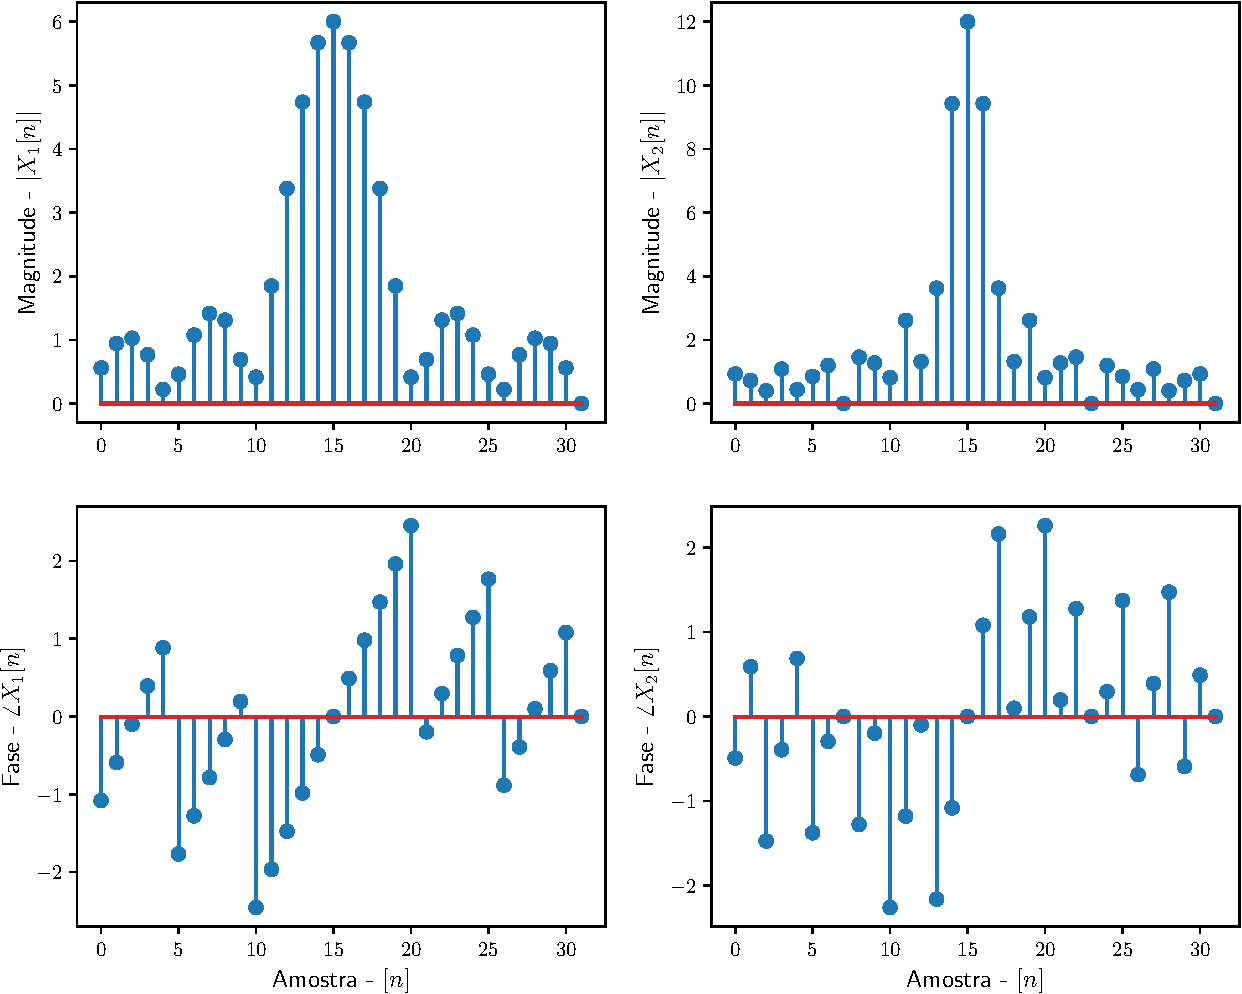
\includegraphics[width=\textwidth]{windowsfft}
	\caption{Visualização das sequências $X_1[k]$ (esquerda) e $X_2[k]$ (direita).}
	\label{fig:windowsfft}
\end{figure}

Nessa visualização, os valores das sequências $X_1[k]$ e $X_2[k]$, que são números complexos, são exibidos através da visualização de magnitude e de fase de cada componente. O formato da magnitude dos sinais exibe a forma da conhecida função $\texttt{sinc} = sin(x)/x$, o que é esperado uma vez que os sinais no domínio do tempo consistem em janelas retangulares.

\subsection{Multiplicação no Domínio da Frequência}

Após o cálculo das transformadas individuais, podemos calcular a transformada resultante ao multiplicar cada sequência \textit{ponto-a-ponto}. O procedimento é bastante simples, e o resultado é exibido na Figura \ref{fig:filterfft} abaixo.

\begin{figure}[ht] \centering
	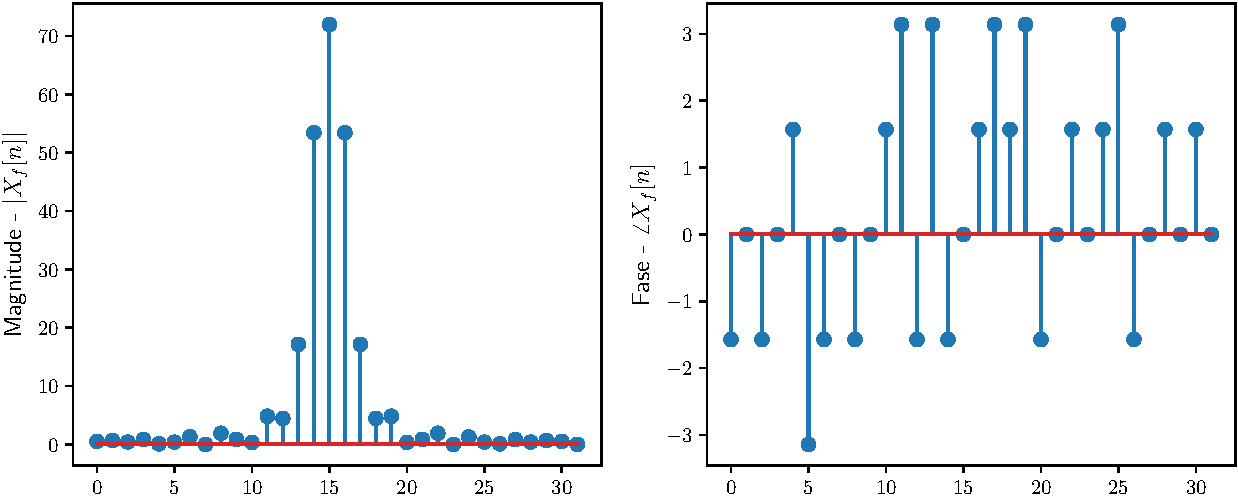
\includegraphics[width=\textwidth]{filterfft}
	\caption{Visualização da sequências $X_f[k] = X_1[k] X_2[k]$.}
	\label{fig:filterfft}
\end{figure}

\subsection{Transformada Inversa de Fourier do Sinal Resultante}

Subsequentemente, é possível analisar o resultado da convolução no domínio do tempo ao realizar a IDFT diretamente à sequência $X_f[k]$. O resultado é demonstrado na Figura \ref{fig:trapez} abaixo.

\begin{figure}[ht] \centering
	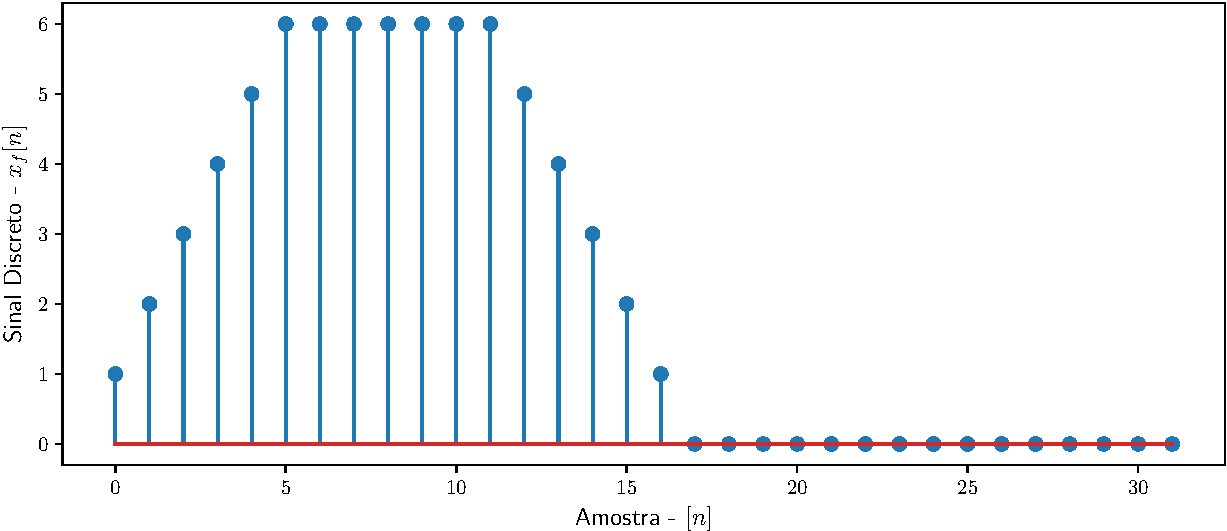
\includegraphics[width=0.8\textwidth]{trapez}
	\caption{Visualização da sequência $x_f[n] = x_1[n] * x_2[n]$.}
	\label{fig:trapez}
\end{figure}

O sinal resultante exibe alguns resultados interessantes. Primeiramente, nota-se que o sinal resultante da convolução, no domínio do tempo, possui exatamente $16$ amostras não-nulas, o mesmo resultado da soma $N_1 + N_2 - 2$, onde $N_1$ e $N_2$ são os tamanhos das respectivas sequências originais. Ademais, o sinal resultante possui um formato trapezoidal cujo topo possui $N_1+1$ amostras de valor $N_1$. Um sinal trapezoidal é um resultado característico da convolução entre dois sinais retangulares, e o mesmo se reduz a um sinal triangular quando os sinais possuem a mesma largura (pois haveria apenas uma superposição completa entre esses sinais).

Finalmente, comparamos o resultado da convolução no tempo através da multiplicação na frequência com o resultado de diretamente computar a convolução discreta no domínio do tempo. As sequências resultantes obtidas são comparadas na Figura \ref{fig:convVsFourier}. A fim de enfatizar possíveis diferenças, a visualização é realizada utilizando um gráfico de linhas, apesar de que os dados em questão ainda sejam discretos. Podemos perceber, pela visualização, que os dois métodos obtiveram praticamente os mesmos resultados, dado a perfeita superposição entre as linhas no gráfico. Portanto, demonstramos a equivalência entre a convolução no tempo com a multiplicação na frequência, além de demonstrar a vantagem computacional dessa abordagem, uma vez que multiplicações são menos custosas que convoluções.

\begin{figure}[ht] \centering
	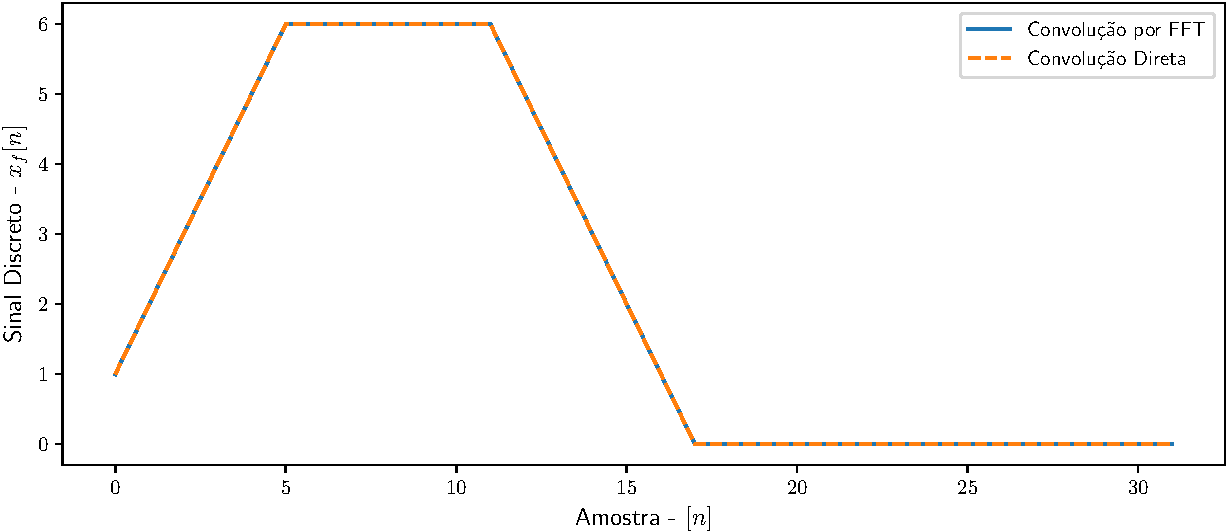
\includegraphics[width=0.8\textwidth]{convVsFourier}
	\caption{Comparação entre o resultado da proposta convolução para os dois métodos citados.}
	\label{fig:convVsFourier}
\end{figure}

% A - Explicações
% ---------------------------------------------------------------
\clearpage
\section*{A - Explicação da FFT e Detalhes de Implementação}

Nessa secção explicamos a formulação matemática do algoritmo de Transformada Rápida de Fourier e apresentamos uma implementação desse algoritmo utilizando a linguagem de programação Python. Tratamos, aqui, exclusivamente do método \textit{Radix-2 Decimation-In-Time} para implementação da transformada rápida. A implementação apresentada fora utilizada nos exercícios anteriores nesse documento.

Considere a definição da Transformada Discreta de Fourier (DFT), dada como:
\begin{equation} \label{eq:dft}
\begin{matrix}
	X[k] = \displaystyle\sum_{n = 0}^{N-1} x[n] W_N^{kn}, & k = 0, 1, \cdots, N-1
\end{matrix}
\end{equation}

\noindent de onde $W_N = e^{-j2\pi / N}$. Podemos, então, particionar o somatório em dois somatórios independentes, sendo o primeiro uma iteração sobre os elementos de índice ímpar e o segundo uma iteração sobre os elementos de índice par da sequência. Ou seja,
\begin{equation} \label{eq:fft02}
\begin{split}
	X[k] &= \sum_{n even} x[n] W_N^{kn} + \sum_{n odd} x[n] W_N^{kn} \\
		 &= \sum_{m = 0}^{(N/2)-1} x[2m] W_N^{k(2m)} + \sum_{m = 0}^{(N/2)-1} x[2m+1] W_N^{k(2m+1)} \\
		 &= \underbrace{\sum_{m = 0}^{(N/2)-1} x[2m] W_{N/2}^{km}}_{X_e[k]} + W_N^{k} \underbrace{\sum_{m = 0}^{(N/2)-1} x[2m+1] W_{N/2}^{km}}_{X_o[k]}
\end{split}
\end{equation}

\noindent onde no último passo fora utilizado $W_N^{2km} = e^{(-j2\pi / N)2km} = e^{(-j2\pi / (N/2))km} = W_{N/2}^{km}$. Agora, sabemos que $X_e[k]$ e $X_o[k]$ ambos são periódicos com período $(N/2)$, o que implica em $X_e[k+N/2] = X_e[k]$ e $X_o[k+N/2] = X_o[k]$. Ademais, temos a propriedade de que $W_N^{k+N/2} = -W_N^{k}$. Portanto, a equação acima pode ser representada pelo par de equações:
\begin{align} 
	X[k] &= X_e[k] + W_N^k X_o[k],\ \ k = 0,1,2, \cdots, \cfrac{N}{2} - 1 \label{eq:fft03a} \\ 
	X\left[ k + \cfrac{N}{2} \right] &= X_e[k] - W_N^k X_o[k],\ \ k = 0,1,2, \cdots, \cfrac{N}{2} - 1 \label{eq:fft03b}
\end{align} 

Portanto, é possível calcular a transformada $X[n]$ utilizando os resultados já computados em $X_e[k]$ e $X_o[k]$. Claramente, também é possível realizar o mesmo particionamento feito em \eqref{eq:fft02} diretamente em $X_e[k]$ e $X_o[k]$, o que implica em que o cálculo da transformada final pode ser realizado de maneira recursiva. Essa abordagem, conhecida como \textit{dividir e conquistar}, reduz o número de computações necessárias ao reaproveitar a solução de subproblemas menores. 

No caso do algoritmo de FFT em discussão, é possível associar as computações à diagramas de fluxos, como exemplificado na Figura \ref{fig:radix2} para uma sequência de tamanho $N=8$. Na Figura \ref{fig:radix2a} temos a estrutura geral da recursividade na solução da FFT, enquanto que a Figura \ref{fig:radix2b} é o diagrama de fluxo que explicita as operações entre os sinais. Nessa estrutura, cada cruzamento entre pares $X_e[k]$ e $X_o[k]$ é denominado de \textit{borboleta}. Por fim, note que o procedimento de recursivamente dividir a sequência acabou causando um ``embaralhamento'' da ordem dos índices na sequência original, apesar de que as transformadas são calculadas na ordem correta. No caso do algoritmo em questão, no entanto, esse ``embaralhamento'' pode ser facilmente calculado ao notar-se que ele correponde à inversão dos bits do índice na sua representação binária.

\begin{figure}[!ht] \centering
	\begin{subfigure}{0.95\textwidth} \centering
		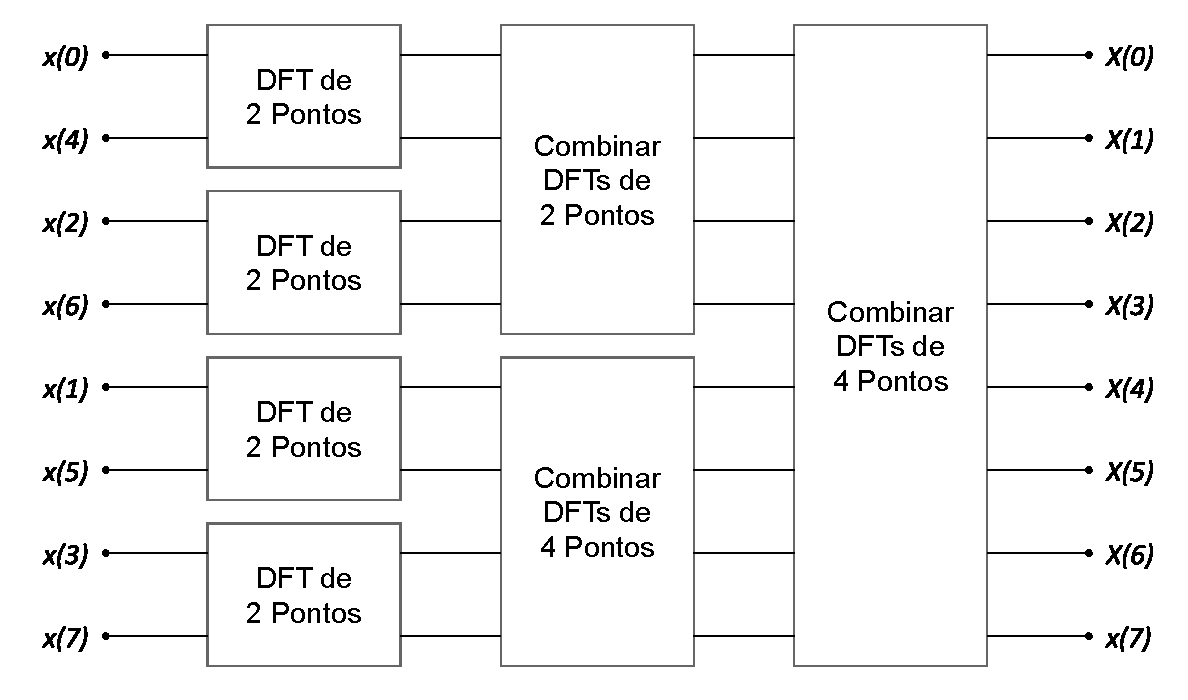
\includegraphics[width=\textwidth]{radix2a}
		\caption{}
		\label{fig:radix2a}
	\end{subfigure}\\
	
	\begin{subfigure}{0.95\textwidth} \centering
		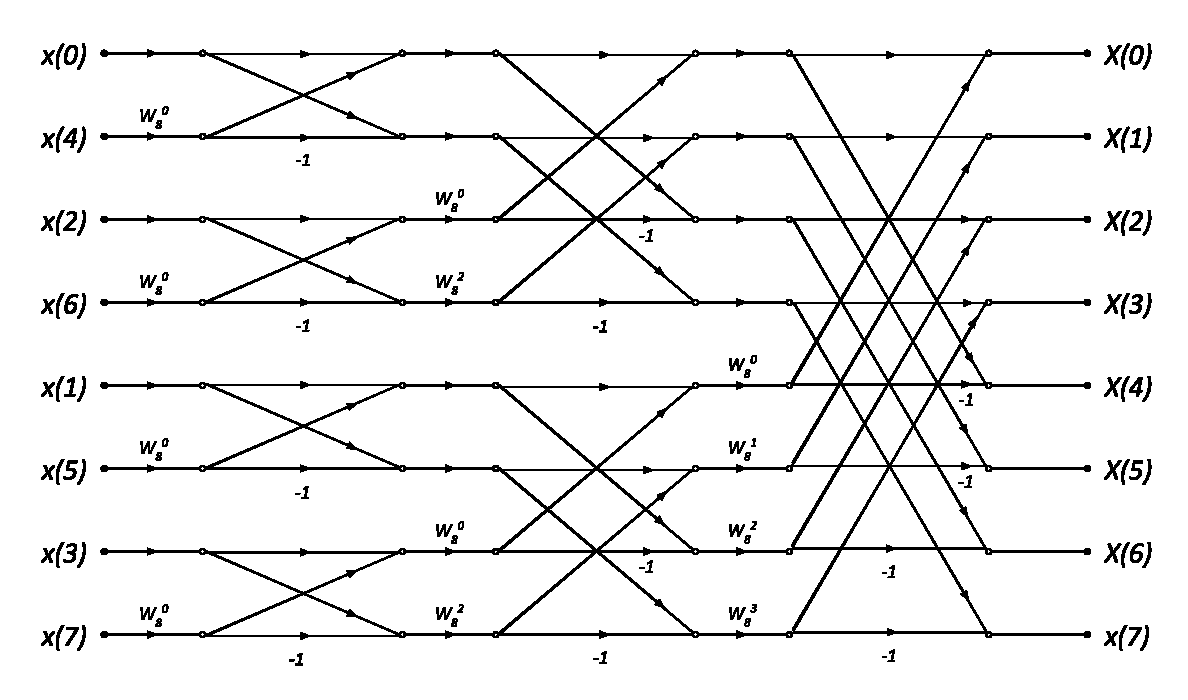
\includegraphics[width=\textwidth]{radix2b}
		\caption{}
		\label{fig:radix2b}
	\end{subfigure}
	
	\caption{Esquemático da TRF pelo algoritmo \textit{Radix-2 Decimal-in-Time}.}
	\label{fig:radix2}
\end{figure}

\subsection{Complexidade Computacional}

Primeiramente, discutimos a complexidade computacional do cálculo da Transformada de Fourier Discreta diretamente pela aplicação da fórmula em \eqref{eq:dft}. Note que por essa fórmula temos um total de $N-1$ adições complexas e $N$ multiplicações complexas (uma multiplicação para cada iteração do somatório), sendo essas operações repetidas para cada diferente valor de $k$. Uma vez que $k = 0, 1, \cdots, N-1$, então teremos um total de $N$ repetições dessas operações, o que resulta em $N^2-N$ adições complexas e $N^2$ multiplicações complexas para o cálculo da transformada discreta. Dessa forma, a complexidade computacional dessa abordagem é dada por
\begin{equation}
	\mathcal{O}\left( N^2-N + N^2 \right) = \mathcal{O}\left( N^2 \right)
\end{equation} 

Agora, consideramos a complexidade do algoritmo de Transformada Rápida pelo método \textit{Radix-2 Decimation-in-Time}. Note que, evidenciado pelo diagrama na Figura \ref{fig:radix2a}, esse algoritmo divide o cálculo da transformada num total de $log_2(N)$ estágios, onde $N$ é o número total de pontos. Para cada estágio, pares periódicos de pontos são combinados de acordo com as equações \eqref{eq:fft03a} e \eqref{eq:fft03b}, o que consiste na operação denominada de \textit{``borboleta''}. Se pré-calcularmos $z_k = W_N^k X_o[k]$, cada \textit{borboleta} consiste em exatamente 1 multiplicação complexa e 2 adições complexas. Uma vez que consistem em cruzamento de pares, cada estágio tem exatamente $N/2$ \textit{borboletas}, o que resulta no total de $N/2$ multiplicações complexas e $N$ adições complexas. Por fim, teremos um total de $(N/2)log_2(N)$ multiplicações complexas e $N log_2(N)$ adições complexas, resultando na complexidade computacional de
\begin{equation}
	\mathcal{O}\left( \cfrac{N}{2} log_2(N) + N log_2(N) \right) = \mathcal{O}\left( N log_2(N) \right)
\end{equation} 

Conclui-se que o algoritmo de Transformada Rápida de Fourier apresenta uma melhora significativa em relação ao cálculo direto, uma vez que $\mathcal{O}\left( N log_2(N) \right)$ cresce muito mais lentamente que $\mathcal{O}\left( N^2 \right)$ para valores muito altos de $N$. 

\subsection{Implementação}

Para este trabalho, o algoritmo de FFT \textit{Radix-2 Decimation-in-Time} fora implementado utilizando a linguagem de programação \textit{Python}. A função de transformação (tanto direta como inversa) é apresentada abaixo:

\begin{lstlisting}[language=Python]
def fft(x_n, inverse=False):
  N = len(x_n)
  W_N = np.exp((-1)**(not inverse) * 2j * np.pi / N)

  x_n = bitrevorder(x_n)

  size = 2
  while size <= N:
    step = size // 2
    for i in range(0, N, size):
      k = 0
      for j in range(i, i + step):
        z_k = (W_N**k) * x_n[j + step]

        x_n[j + step] = x_n[j] - z_k
        x_n[j] 	      = x_n[j] + z_k
				
        k += N // size
    size *= 2

  return (1/N)**inverse * x_n
\end{lstlisting}

Essa implementação é bastante prática. Inicia-se ao realizar o reordenamento dos índices da sequência original, utilizando a função $\texttt{bitreorder(.)}$. Logo após essa operação, inicia-se um \textit{while-loop} para iterar sobre todos os possíveis níveis de recursividade. Dentro desse laço, dois \textit{for-loops} são implementados: o primeiro irá iterar sobre os \textit{``pontos de início''} das \textit{borboletas}, enquanto o laço seguinte irá iterar sobre todos os pares de borboletas a partir daquele ponto. Para cada iteração dos laços aninhados, a transformada é calculada utilizando exatamente a fórmula exposta em \eqref{eq:fft03a} e \eqref{eq:fft03b}, sendo $z[k] = W_N^k x[n+S/2]$ uma variável auxiliar.

O cálculo da Transformada Inversa de Fourier segue exatamente o mesmo formato de uma Transformada Direta, porém temos que $W_N = e^{j2\pi/N}$. A implementação de tal método, utilizando a função já apresentada, consistiu apenas em adicionar uma variável booleana (a variável $\texttt{inverse}$) que \textit{``ativa''} os fatores de fase adequado e a normalização do sinal calculado para obter o resultado da transformação inversa. Por fim, enfatiza-se que outras funções auxiliares utilizadas nos exercícios, e que não foram explicitadas nesse relatório, também se encontram implementadas no arquivo de código \texttt{FFT.py} que o acompanha.

% ---------------------------------------------------------------
% End document
% ---------------------------------------------------------------

\end{document}

%%%%%%%%%%%%%%%%%%%%%%%%%%%%%%%%%%%
%% Drafts:
%%%%%%%%%%%%%%%%%%%%%%%%%%%%%%%%%%%
%%%%% Figure:
% \begin{figure}[ht]
%   \centering
%   \includegraphics[trim={0cm 0cm 0cm 0cm},clip,scale=1]{nameFigure}
%   \caption{Caption of the figure.}
%   \label{fig:nameFigure}
% \end{figure} \vskip0.25cm
%
%%%%% Equation:
% \begin{equation} \label{eq:nameEquation}
% \begin{split}
%    X = 1 + 1
% \end{split}
% \end{equation} \vskip0.25cm
%
%%%% Table:
% \begin{table}[hp]
%   \centering
%   \begin{tabular}{l | c c }
%   Principal & Coluna1 & Coluna2 \\
%   \hline 
%   ABC & 1 & 2 \\
%   DFG & 3 & 4 \\
%   HIJ & 5 & 6 \\
%   \end{tabular} 
%   \caption{Caption of the table.}
%   \label{table:nameTable} 
% \end{table} \vskip0.25cm

%\begin{figure}
%    \centering
%    \begin{minipage}[t][6cm][t]{.48\textwidth}
%	\begin{tikzpicture}
%	  \begin{axis}[enlargelimits=false, scale only axis, axis on top, width=0.8\textwidth,
%	  	xlabel={$u$ unemployment}, ylabel={$\pi$ inflation}]]
%		\addplot graphics [xmin=0,xmax=96,ymin=0,ymax=96] {chapter3/report_ch3_1_1};
%	  \end{axis}
%	 \end{tikzpicture}
%	\end{minipage}%
%	\hfill
%	\begin{minipage}[t][6cm][t]{0.48\textwidth}
%	\begin{tikzpicture}
%	  \begin{axis}[enlargelimits=false, scale only axis, axis on top, width=0.8\textwidth,
%	  	ylabel={$\pi$ inflation}]]
%		\addplot graphics [xmin=0,xmax=96,ymin=0,ymax=96] {chapter3/report_ch3_1_2};
%	  \end{axis}
%	\end{tikzpicture}%
%	\vspace{.6ex}
%	\begin{tikzpicture}
%		\begin{axis}[enlargelimits=false, scale only axis, axis on top, width=0.8\textwidth,
%	  	xlabel={$u$ unemployment}, ylabel={$\pi$ inflation}]]
%		\addplot graphics [xmin=0,xmax=96,ymin=0,ymax=96] {chapter3/report_ch3_1_3};
%		\end{axis}
%	\end{tikzpicture}
%	\end{minipage}%	
%    
%    \caption{A}
%    \label{fig:regulator01}
%\end{figure}